\documentclass{article}
\usepackage{parskip}
\usepackage[utf8]{inputenc}
\usepackage{hyperref}
\usepackage[hidelinks]{hyperref}
\hypersetup{
    colorlinks=true,
    linkcolor=blue,
    filecolor=magenta,      
    urlcolor=cyan,
    pdftitle={Overleaf Example},
    pdfpagemode=FullScreen,
    }
\urlstyle{same}
\title{MICROSOFT CYBERSECURITY ENGAGE 
Project: Attack Navigator
}
\author{\href{https://www.linkedin.com/in/mitarth-arora-27300920a/}{\bf Mitarth Arora, IIT Jodhpur} \\}
\usepackage{graphicx}
\graphicspath{ {./} }
\usepackage[usenames,dvipsnames]{color}
\usepackage{multirow}
\usepackage[export]{adjustbox}

\definecolor{function}{RGB}{97, 175, 239}
\definecolor{attribute}{RGB}{204, 65, 37}
\definecolor{class}{RGB}{241, 194, 50}
\definecolor{grey}{RGB}{171, 178, 191}

\begin{document}

\maketitle
\section{Abstract}
This research paper addresses the influence of malwares on cyber-attacks and cyber-defense on the institutions of national security and importance. It first analyses trends in cyber-weapons and how it fits into these trends.

Attack navigator is a superb cybersecurity gadget built out in this project to secure the higher military organisations in delivering or receiving out the essential data and messages over the network.We have built Attack Navigator based on the concept of MITRE ATT\&CK through which we can understand how the system is being attacked and what the attacker might do next ? This approach encrypts the data by computing substitution cipher via an encryption algorithm \textbf{encryption.py} which is not that easy to crypt-analyze. Basically, we have substituted each character in the data with a different character whose selection is done randomly. Therefore, in case, if someone has the access to our operating system, then likewise he/she will not be able to grasp any portion of the data. Hence, our data system of military organisations remains out to be guarded.

% A custom function \textcolor{function}{\textbf{visualise\_audio}} for plotting the subplots for each signal.\\

\section{Methodology and Assumptions}

Military practitioners have been excited by the usage of the term ‘cyber war’ for some years now. Influence of technology on warfare is rising, and cyber capabilities only accentuate the reality. It is sometimes speculated that information technology and cyber might well determine the victor in the digital battlefield of tomorrow. Technological breakthroughs have radically transformed and impacted the doctrinal, organisational and strategic aspects of combat. Information technologies, sensors, miniaturisation and pervasive wireless connectivity have created a whole new realm of combat by way of ‘cyber space’ and put warfare on the cusp of an epochal change from the conventional to an information-based virtual era. This wave of cyber-driven change is radical, sweeping and imaginative, necessitating a relook at old strategic plans and to map out a new route for operational enhancement and enhanced tactical efficiency. Cyberspace and cyber power provide a whole new set of technology solutions to some of the challenges of modern combat of the government and country.

The effects of the deployment of cyber power and criminality for offensive operations may vary in intensity, lethality, intent or geographical distribution and can appear in complex, dynamic and unforeseen ways, with far-reaching tactical and strategic ramifications. We need to establish and promulgate our policy and paper out for capacity building of cyber deterrence related strategy, and a doctrine for our armed forces.Accordingly, figuring out the necessity and requirement of the cybersecurity in this sector. I have begun out a notion of \textbf{Attack Navigator}.

Also during this whole project, I have gone through over the number of research papers and all of them have been properly cited out towards the end of the report. 

\section{Cyber Detterence and it's Challenges}

Before starting out with this very important topic, it is very crucial on our end to know that what exactly Cyber Detterence is ? 

Whether a cyber war takes happen or not, offensive cyber-attacks are increasingly being considered as a hazard to national security. This does not mean that there is now absolute clarity in reacting to these dangers, merely that the exploitation of cyberspace is reaching levels that imperil essential national interests.

Deterring threats instead of waging harmful conflicts has been a persistent strategic objective through the centuries. Deterrence is the process of deterring or restricting someone—in international politics, generally a nation-state—from doing unwelcome acts, such as an armed attack.Conventional deterrence was believed more difficult to implement than nuclear deterrence because whereas nuclear weapons have a well defined end result, the outcome of conventional combat is unpredictable. Nevertheless, conventional deterrence is still regarded a key aspect of national plans.

\subsection{Defining the Cyber Threats to be Deterred}
Cyber threats may take different forms, from malware, phishing, identity theft, denial of service, ransomware to espionage and disruption of a nation's key infrastructure. Unfortunately, it is nearly hard to discourage all forms of threats, and in designing a national plan for cyber deterrence, there must be a clearly defined approach.

The first stage is to define the cyber risks that would represent a danger to national security and armed forces in closer focus. Attacks that undermine the integrity of important data; and efforts to provoke loss of faith in the government or disrupt societal cohesion.

A national reaction must be targeted largely against state-sponsored attacks, whether carried out directly or through state proxies. We have to recognise the truth that individual criminal hackers cannot be effectively discouraged, and it would be futile to adopt a 'whack-a-mole' approach against all cyber threats. States are the more rational actors in international affairs, and a cost and benefits strategy is easier to employ to them than to a collection of terrorists or cyber criminals.

\subsection{Challenges of Cyber Deterrence}
A deterrence strategy depends on the power of a state to restrict an opponent by threats, coercion, or reward. There is a great lot of disagreement on whether the nature of threats in cyberspace can truly be discouraged and whether we are considering adapting a technique that works effectively in the nuclear arena to an altogether different form of danger. Some of the obstacles to the notion of cyber deterrence are covered here.

\begin{itemize}
\item \textbf{Attribution} is likely the toughest problem. Nations must be clear about the identity of the perpetrator of a cyber assault so that their counter operations are not misdirected. This is not straightforward since locations may be faked, identities masked, and the nature of cyberspace means that assaults can be launched from any geographical area. In addition, misleading flags might be deployed to fool or misguide attempts to identify the attackers.
\item Another issue to cyber deterrence is the \textbf{unpredictability of the effect}. Nuclear deterrence succeeded in army because the capabilities of either side were recognised, as was the devastating power of atomic bombs. National cyber capabilities are carefully guarded, and there is little clarity about how a cyber response will effect the opponent.
\item \textbf{Understanding Adversary Motives and Level of Risk Tolerance} is also a challenge as the human and military abilities to deter each group of cyber adversaries
will vary as per the need and requirements.
\end{itemize}

\subsection{Components of Cyber Deterrence}
There are two fundamental approaches to deterrence; \textbf{Denial and Punishment}.
\begin{itemize}
\item\textbf{Cyber deterrence through denial} involves the hardening of our vital information infrastructure to the point that the enemy thinks that targeting such systems would produce few benefits. It is a well-known truth that current attacks in cyberspace have a particular edge over defensive measure. Despite this, security of networks, redundancy in systems, usage of trustworthy technology, and defending forward might offset some of the limitations of cyber defence.
\item\textbf{Deterrence by punishment} aims to prohibit an adversary from carrying out unwanted activities by the prospect of imposing excessive costs. It must be clearly emphasised that cyber assaults which endanger national security will always be reacted against. And this response is not necessarily confined to operations in cyberspace but encompasses military, economic, diplomatic, and legal measures.
\end{itemize}

\subsection{Conclusion over Cyber Deterrence}
There are various hurdles to deterrence in cyberspace, but that should not preclude us from holding hostile actors accountable for their conduct. National Military Forces commitment to forcefully respond to threats to national security must be clearly expressed through an outlined cyber deterrence plan. The various government authorities should be charged to design this plan in cooperation with other government agencies.

Deterrence is a mix of communication, credibility, and competence. Downplaying major occurrences, an unwillingness to respond, and capabilities flaws in cyber power might have catastrophic effects. A national cyber deterrence plan may not be a full answer to combatting state-sponsored cyber assaults, but it is surely an essential element and also the need of the hour.

\section{Legal and Treaty Assumptions}

Addressing the gaps and obstacles in international laws outlined , it is vital to create a digital environment where duties and expectations for responsible state behaviour are both recognised and accepted.

This clarity is vital for pushing back against harmful tendencies in the weaponization of the online world, where ambiguity is too frequently exploited to irresponsible goals that can threaten the safety, security, and trust of individuals and armed forces and organisations.

Given current trends, it is clear that international law either

(a) does not sufficiently prohibit some of the most egregious and unwanted cyberactivity, including systemic cyber operations targeting individual users or their infrastructure below the use of force threshold, or

(b) provides a “patchwork” of contested rules (and meanings) resulting in insufficient and or ineffective regulation or deterrence of or consequences for unwanted activity.

To remedy this, this paper has recommended and promoted out the development of clear and binding legal obligations for cyberspace for all the stakeholders needed for this big change in society and to meet out the need of an hour.

Until governments are more upfront about their views on how international law applies to their cyber activities, and explain their methods, the findings below concerning the application of international law to states’ cyber operations are unavoidably cautious. The following conclusions and recommendations are a product of considerable study and discussions of various number of research papers.

\subsection{Recommendations over the International Law}

\begin{itemize}
\item International laws must be \textbf{uniform} and applicable out to all the states’and military operations in cyberspace on a same profile 
\item In the absence of relevant treaties other than the UN Charter, existing customary international law must be resorted to as a basis for the law applicable in cyberspace. Publicly available state practise related especially to cyberspace is currently scant. But as with any other state activity, existing principles and norms of international law are applicable to state actions in cyberspace, unless there is known methods with \textbf{opinio iuris} to suggest that a relevant principle or rule is not applicable.
\item The principle of sovereignty applies in relation to states’ cyber activities, as it applies in the non-cyber context. The principle has \textbf{legal consequences}.
\item A state’s power and jurisdiction apply in respect to cyber infrastructure and operations within its territory, as they do to other subjects. Territorial sovereignty and the independence of a state’s powers vis-à-vis other states are therefore relevant.
\end{itemize}

\subsection{Recommendations to National Government}

\begin{itemize}
\item States need to make an educated choice as to where their own stance rests on the application of international law to cyber activities. Intelligence as well as military agencies and foreign services inside a state need to talk with one voice.
\item The UN offers \textbf{one platform} for discussion. Further interaction across various groupings of nations, military organisations , academics, private-sector organisations and civil society on these concerns would also be useful, building on the work in come and other efforts.
\item Instead, subsequent discussion should focus on how the regulations relate to real cases of \textbf{nation-sponsored} cyber activities. There may be greater commonality regarding concrete applications of the law.
\item The possibilities of an \textbf{universal treaty} in this area are far off. There may be advantage in striving for agreement on particular norms, for example on due diligence and a prohibition on attacking critical infrastructure, before discussing larger principles of law and treaties.
\end{itemize}

\section{Solution Architecture}
Here we have explained out our whole work system in the form of \textbf{flowchart} shown below:

\maketitle
\begin{figure}[htp]
    \centering
    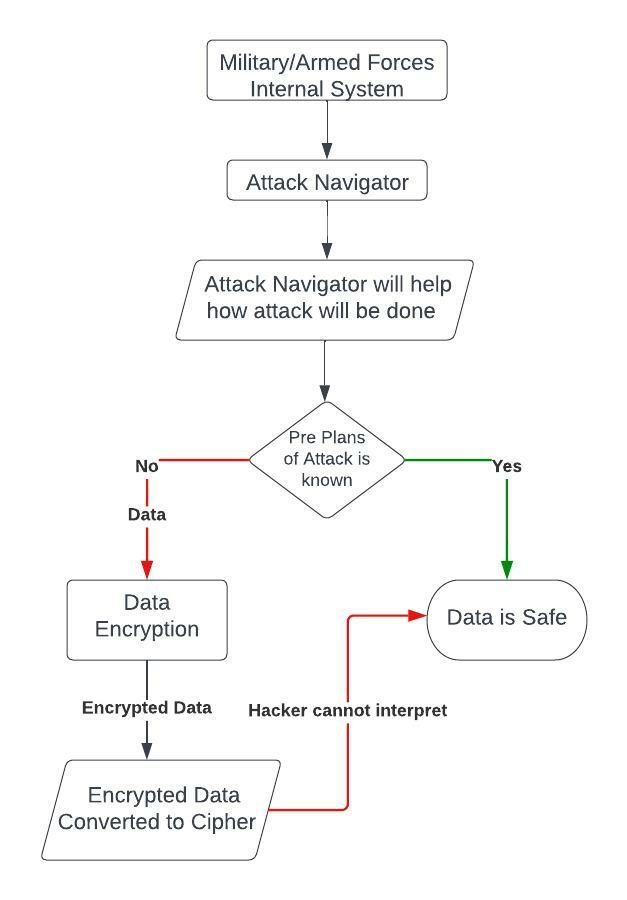
\includegraphics[width=9.80cm]{Flow Chart Attack Navigator.jpeg}
    \caption{System Architecture}
    \label{fig:galaxy}
\end{figure}



\section{Functioning Prototype}
The Attack Navigator is designed to provide basic navigation and annotation of Attack matrices, something that people are already doing today in tools like Excel. We've designed it to be simple and generic - you can use the Navigator to visualize your defensive coverage, your red/blue team planning, the frequency of detected techniques or anything else you want to do. The Navigator doesn't care - it just allows you to manipulate the cells in the matrix (color coding, adding a comment, assigning a numerical value, etc.). We thought having a simple tool that everyone could use to visualize the matrix would help make it easy to use Attack.

The principal feature of the Navigator is the ability for users to define layers - custom views of the Attack knowledge base - e.g. showing just those techniques for a particular platform or highlighting techniques a specific adversary has been known to use. Layers can be created interactively within the Navigator or generated programmatically and then visualized via the Navigator.

\begin{center}
   \textbf{Github Link of the Project : -}
\href{https://github.com/mitarth-arora/Attack-Navigator.git}{View on Github}
\end{center}
\section{Defining Benchmarks of Success}
\begin{itemize}
\item We have developed a framework which tracks adversarial technique that are used during different stages of a cyber attack.
\item An intent-based response uses out a dynamic and contextual kill chain framework that can help our organization to correlate security incidents and to identify a large scope of attacks on military databases. 
\item  This framework supports governance, risk management, understanding of attacker behaviour, understanding how to classify and mitigate threats and ultimately help us in understanding adversaries and the methods they are likely to use in order to compromise our very important military data as well as it can be used in the protection of any government entities. 
\item When we understand this sequence of the tactics which represents what an adversary is trying to accomplish at the stage of an incident as cyber security expert, we have an opportunity to anticipate an adversary's next move and break the kill chain.
\item  In case we are not able to break the kill chain and our system has got a external remote access, then also our important military databases is not that easy to crypt-analyze and crack the substitution cipher.
\item In the worst case if by chance it is cracked then also we will receive out the complete information of the unauthorised access of our important systems and network. Then we as Cyber security experts can change our plan of action within the same set of duration.
\end{itemize}

\section{Acknowledgement}
First of all my sincere thanks to almighty God without whose blessings this project would have been an indefinite task. I would also want to thank the team at Microsoft and Ace Hacker including Mr.Vivek Shangari and all the respective dignitaries for giving out their so much valuable time and for bringing out such a great opportunity for us and with that also want acknowledge the following links and papers that have helped me to
gain some knowledge for this report. 

Finally, I would also like to thank my parents and friends who helped me a lot in finalizing this project within the time frame.
I have listed all links from which educational data/framework were being used. In case of any missing links, I would like to thank the owner and promise to abide by the fact that this educational content is in fair use without violating the copyright rules.

\section{References}
\begin{itemize}
\item \href{https://www.vifindia.org/sites/default/files/Credible-Cyber-Deterrence-in-Armed-Forces-of-India_0.pdf}{https://www.vifindia.org/sites/default/files/Credible-Cyber-Deterrence-in-Armed-Forces-of-India_0.pdf}
\item\href{
https://www.sciencedirect.com/science/article/abs/pii/S0267364910000506
}{
https://www.sciencedirect.com/science/article/abs/pii/S0267364910000506
}
\item\href{https://www.jstor.org/stable/pdf/resrep13817.9.pdf}{https://www.jstor.org/stable/pdf/resrep13817.9.pdf}
\item\href{https://www.inss.org.il/wp-content/uploads/2017/02/FILE1333533336-1.pdf}{https://www.inss.org.il/wp-content/uploads/2017/02/FILE1333533336-1.pdf}
\item\href{https://docs.servicenow.com/bundle/paris-security-management/page/product/threat-intelligence/concept/about-mitre-attack.html}{https://docs.servicenow.com/bundle/paris-security-management/page/product/threat-intelligence/concept/about-mitre-attack.html}
\item\href{https://www.un.org/disarmament/wp-content/uploads/2019/12/protecting-people-in-cyberspace-december-2019.pdf}{https://www.un.org/disarmament/wp-content/uploads/2019/12/protecting-people-in-cyberspace-december-2019.pdf}
\item\href{https://www.chathamhouse.org/sites/default/files/publications/research/2019-11-29-Intl-Law-Cyberattacks.pdf}{https://www.chathamhouse.org/sites/default/files/publications/research/2019-11-29-Intl-Law-Cyberattacks.pdf}
\item\href{https://www.jstor.org/stable/40664079?seq=1}{https://www.jstor.org/stable/40664079?seq=1}
\item\href{https://carnegieendowment.org/2021/05/19/un-struggles-to-make-progress-on-securing-cyberspace-pub-84491}{https://carnegieendowment.org/2021/05/19/un-struggles-to-make-progress-on-securing-cyberspace-pub-84491}
\item\href{https://acehacker.com/microsoft/cybersecurity/resources/The-History-of-Stuxnet.pdf}{https://acehacker.com/microsoft/cybersecurity/resources/The-History-of-Stuxnet.pdf}
\item\href{https://acehacker.com/microsoft/cybersecurity/resources/Stuxnet-and-Its-Hidden-Lessons-on-the-Ethics-of-Cyberweapons.pdf}{https://acehacker.com/microsoft/cybersecurity/resources/Stuxnet-and-Its-Hidden-Lessons-on-the-Ethics-of-Cyberweapons.pdf}
\item\href{https://acehacker.com/microsoft/cybersecurity/resources/Shadows-of-Stuxnet.pdf}{https://acehacker.com/microsoft/cybersecurity/resources/Shadows-of-Stuxnet.pdf}
\end{itemize}
\centering \textbf{END OF THE REPORT}
\end{document}



